\section{Experiments}

\subsection{Setting warm-up and simulation times}

\begin{minipage}{.6\textwidth}
  In order to define the required warm-up period, we plotted the response time as a function of the simulation time for 10 different runs. The runs were configured in order to represent a worst-case scenario: $\lambda_V=1.3, \lambda_N=0.1,\pi_C=0.1,\mu_K=0.2,\mu_C=1.5$. An example of the plots can be seen in the picture on the right, where simple normal orders are shown. From the plot we can see that the mean starts converging at around 30000m therefore we chose 50000m in order to have some safety margin. We can afford this since running the simulations is quite inexpensive.
\end{minipage}
\begin{minipage}{.4\textwidth}
  \centering
  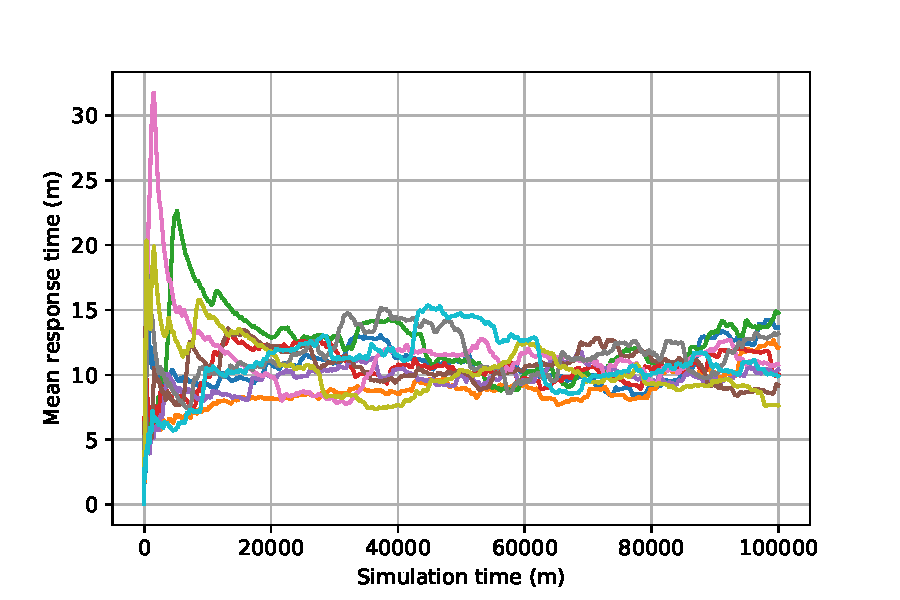
\includegraphics[width=\textwidth]{figs/warmup_definition.pdf}
  \label{fig:warmup}
\end{minipage}

After having chosen the warm-up period, the simulation time was chosen as to have both a high level of accuracy and a small execution time. The value of 500000m has hence been selected since it provides a confidence interval around 2\% with 90\% confidence in the above worst-case scenario.

\subsection{Steady-state analyses}

\subsubsection{2kr analysis}\label{sec:2kr}
In order to grasp the factors contribution to the customers experience, we computed a number of 2$^k$r (r = 5) factorial analysis. In these analyses, we took into 
consideration the following factors in the FIFO kitchen and exponential service and inter-arrival rates scenario: 
\begin{itemize}
  \item A = normal customers rate (VIP rate is set as to keep the total rate constant) $[0.1, 1.2]$
  \item B = odds of an order being a Compound one $[0.1, 0.3]$
  \item C = kitchen Rate $[0.45, 0.6]$
  \item D = cashier Rate $[1.5, 2]$
\end{itemize}
Please note that A is, in reality, a measure of the number customers 
over the total, ranging from ~10\% to ~90\%.

After having run the analyses, we visually checked the residuals' hypotheses for every metric through the related QQ-plot, scatter and lag plots. In the case of queue lengths, few tweaks needed to be made since the residuals QQ-plot was showing lighter tails. The solution was to run the analysis on the log of the queue length. This highlights the non-linear relationship of the queue length with the other factors.

After analyzing all of the metrics, we found no strange behaviour. Therefore, for the sake of brevity, we will only report the most interesting results we found:
\begin{itemize}
  \item the cashier rate has a negative impact ($-0.159 \pm 0.01$, with an explained 92\% variability) on the advantage of VIP customers 
    on normal customers since an increase of it implies lower queuing and thus 
    a more ``equal'' waiting time between VIP and normal customers.
  \item parameter A has a negative contribution on the advantage of VIP       
    customers on normal customers ($-0.0463 \pm 0.0008$, with an explained 7.82\% variability). This is somehow counter-intuitive since we 
    expected the VIP advantage to increase when fewer VIP customers were present.
    However, this results highlights the phenomenon of ``quasi-starvation''
    happening to normal customer with a very high number of VIP customers. In fact, on the one hand, if VIP customers are the great majority, normal customers experience huge waiting times due to too many VIP arrivals jumping in queue in front of them. On the other hand, if normal customers are the great majority: VIP customers are serviced very fast, but normal user are no more ``starved'' by VIPs. 
    This phenomenon is further investigated in \cref{sec:vip_rate}.
  \item the cashier rate has a negligible influence on the kitchen queue length.  
    This phenomenon will be further investigated in \cref{sec:cashier_no_infl}.
\end{itemize} % si può tagliare ancora se serve

\subsubsection{Kitchen Queue Comparison}

In this section we want to assess whether enforcing a priority queue also in the kitchen brings any perks. In order to get that results we observe the trajectories of the \emph{compoundResponseTimeRatio} statistic (i.e. the advantage of being a VIP customer over a normal customer when the order is compound) in both FIFO and priority queue cases, varying the ratio of compound orders.

\begin{figure}[h!]
    \centering
    \begin{minipage}{0.48\textwidth}
      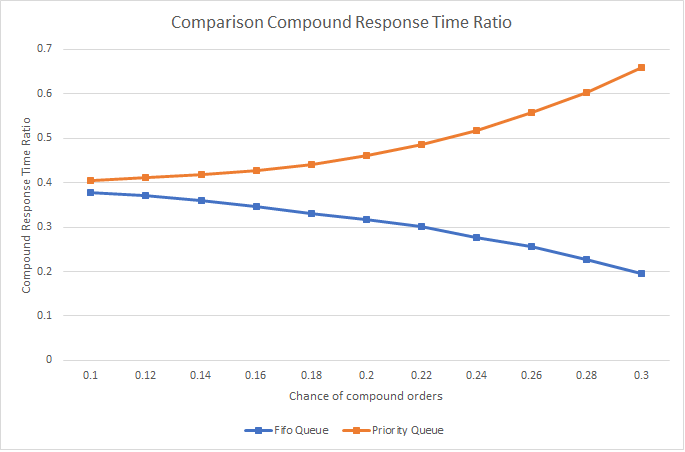
\includegraphics[width=\textwidth]{figs/comparisonQueue.png}
      \caption{VIP advantage over normal for both FIFO and priority queue at the kitchen at different $\pi_C$ ($\lambda_N=1,\lambda_C=0.2,\pi_C={{0.1..0.3 \text{ step } 0.02}}, \mu_K=0.45, \mu_C=1.5$).}
      \label{fig:comp_kitc}
    \end{minipage}\hspace{0.03\textwidth}
    \begin{minipage}{0.48\textwidth}
      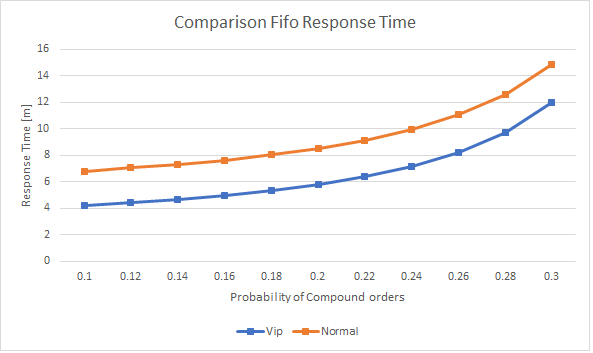
\includegraphics[width=\textwidth]{figs/comparisonFifoKitchen.png}
      \caption{Response time for VIP and normal customers with FIFO queuing at the kitchen at different $\pi_C$ ($\lambda_N=1,\lambda_C=0.2,\pi_C={{0.1..0.3 \text{ step } 0.02}}, \mu_K=0.45, \mu_C=1.5$).}
      \label{fig:fifokitchen-constant}
    \end{minipage}
\end{figure}

\begin{figure}[h!]
  \centering
  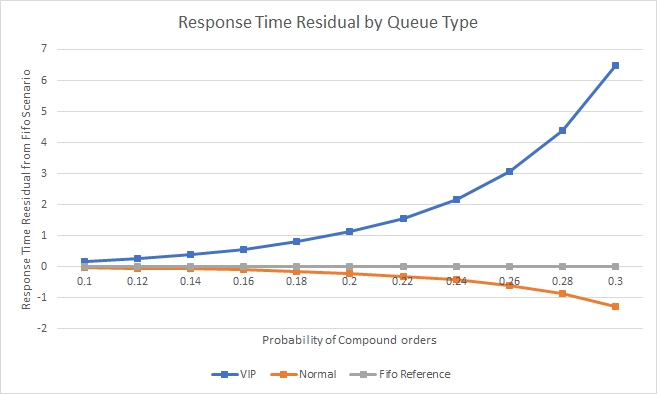
\includegraphics[width=0.6\textwidth]{figs/responseTimeResidualKitchen.png}
  \caption{Residual Response time for Normal and VIP users from what they should expect from a FIFO Scenario in the kitchen($\lambda_N=1,\lambda_V=0.2,\pi_C={{0.1..0.3 \text{ step } 0.02}}, \mu_K=0.45, \mu_C=1.5$).}
  \label{fig:residual}
\end{figure}

In \cref{fig:comp_kitc}, we can clearly see that, in the FIFO case, by increasing the number of compound orders, VIP users tend to lose the ``advantage'' obtained during the cashier service. So, indeed, by using a priority queue in kitchen we can provide an even more privileged service. 

\cref{fig:fifokitchen-constant} highlights even more this phenomenon: in the FIFO scenario, the percentage benefit is reduced since the difference is constant (e.g., around 2m in this scenario), while the response times increase due to higher utilization.

Finally, we would like to be certain that introducing priority queuing at the kitchen does not affect the normal customers' response times too much. This is done in \cref{fig:residual}, where we plotted the difference between recorded response times from FIFO and priority, so that to quantify the time advantage of introducing the priority queuing. From the figure, you can see how introducing priority queuing can bring to great time savings for the VIPs, while not hurting the normal customers too much (e.g., at 26\% compound orders, the VIP mean response time is reduced by 3 minutes while the normal users experience just an half a minute difference). 

\subsubsection{System Response to different Workloads}

\begin{figure}[H]
  \begin{minipage}{0.48\textwidth}
    \centering
    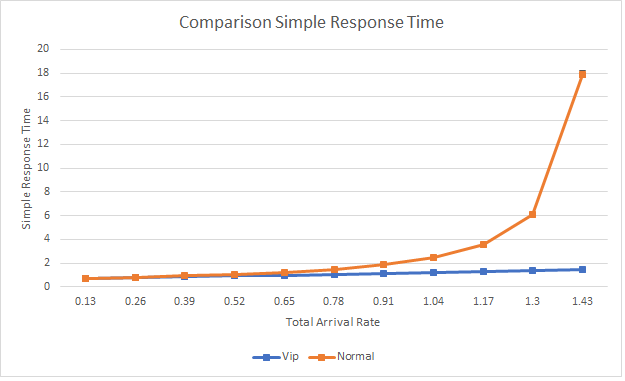
\includegraphics[width=\textwidth]{figs/workloadSimple.png}
    (a)
  \end{minipage}\hspace{0.03\textwidth}
  \begin{minipage}{0.48\textwidth}
    \centering
    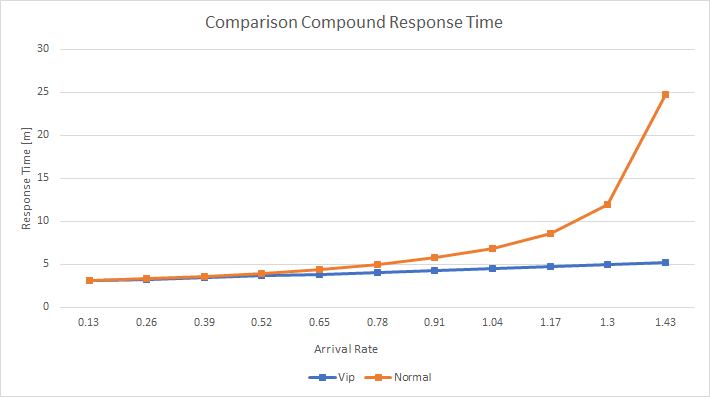
\includegraphics[width=\textwidth]{figs/workloadCompound.png}
    (b)
  \end{minipage}
  \caption{Mean response times for both simple (a) and compound (b) orders of both VIP (blue) and normal (orange) customers by varying total arrival rate. ($\lambda_N={{0.1..1.1 \text{ step } 0.1}},\lambda_V=0.3*\lambda_N,\pi_C=0.2, \mu_K=0.45, \mu_C=1.5$). Note that the Inter-Arrival rate for the kitchen with this configuration is actually 0.2 * "value showed in the x axis".}
  \label{fig:workload}
\end{figure}

In \cref{fig:workload}, the response time for all four kind of orders are shown at different arrival rates.
An interesting, but also expected from QT, aspect is that after a certain threshold of Arrival Rate, that is around 1.3, the Normal response time, for both Simple and Compound orders, explodes.

\subsubsection{VIP Rate study}\label{sec:vip_rate}

One thing that should be taken into consideration when fine-tuning the system is the amount of allowed VIP customers. Of course if all customers were VIP, they would gain little to no benefit and chances are that the few normal customers that arrive will experience a vary bad service. Therefore, it is interesting to study the response of the system at varying percentages of VIP customers in order to find an ``optimal'' value, i.e. one such that VIP benefits are preserved and normal customers are served in a reasonable time. Such study was carried out with a full factorial analysis, varying the percentage of VIP customers.

\begin{figure}[H]
  \begin{minipage}{0.48\textwidth}
    \centering
    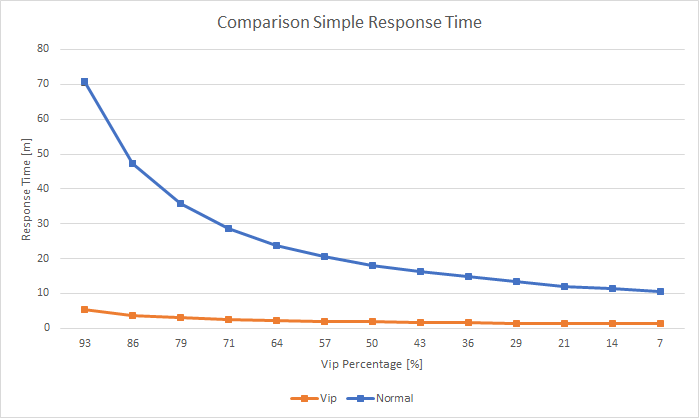
\includegraphics[width=\textwidth]{figs/comparisonSimpleResponseTime.png}
    (a)
  \end{minipage}\hspace{0.03\textwidth}
  \begin{minipage}{0.48\textwidth}
    \centering
    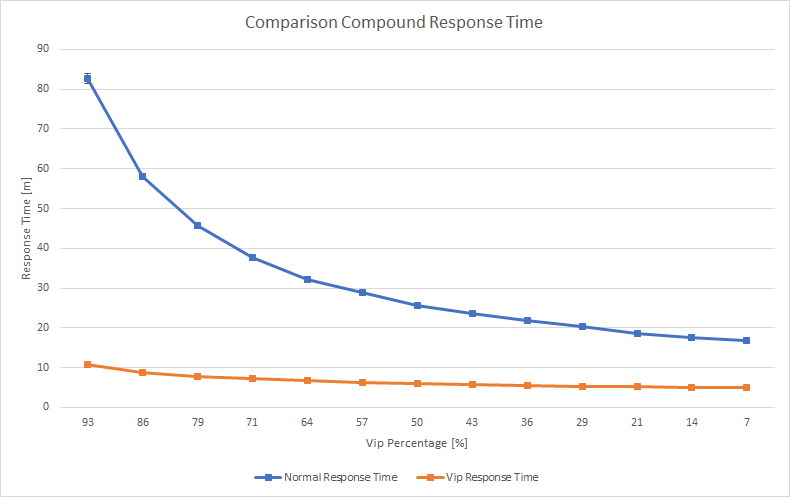
\includegraphics[width=\textwidth]{figs/comparisonCompoundResponseTime.png}
    (b)
  \end{minipage}
  \caption{Both VIP and Normal Response Time at the cashier (a) and kitchen (b) ($\lambda_N={{0.1..1.3 \text{ step } 0.1}},\lambda_V=1.4-\lambda_N,\pi_C=0.2, \mu_K=0.45, \mu_C=1.5$).}
  \label{fig:comp_resp_time}
\end{figure}

\begin{figure}[h!]
  \centering
  \begin{minipage}{0.48\textwidth}
    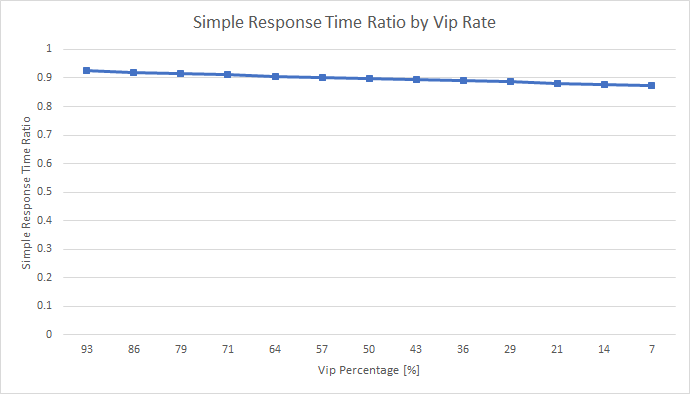
\includegraphics[width=\textwidth]{figs/simpleResponseTimeRatio.png}
    \caption{VIP advantage over Normal at the cashier($\lambda_N={{0.1..1.3 \text{ step } 0.1}},\lambda_V=1.4-\lambda_N,\pi_C=0.2, \mu_K=0.45, \mu_C=1.5$).}
    \label{fig:simpleResponseTimeRatio}
  \end{minipage}\hspace{0.03\textwidth}
  \begin{minipage}{0.48\textwidth}
    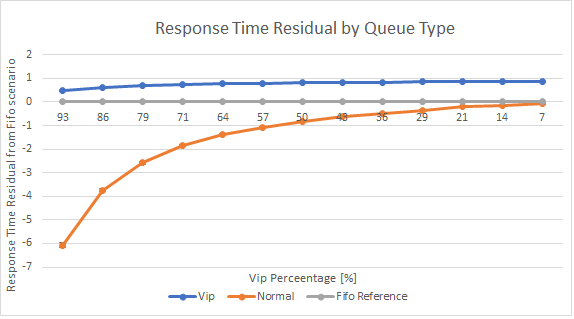
\includegraphics[width=\textwidth]{figs/responseTimeResidualCashier.png}
    \caption{Residual Response time for Normal and VIP users from what they should expect from a FIFO Scenario ($\lambda_N={{0.1..1.3 \text{ step } 0.1}},\lambda_V=1.4-\lambda_N,\pi_C=0.2, \mu_K=0.45, \mu_C=1.5$).}
    \label{fig:residual-cashier}
  \end{minipage}
\end{figure}

In \cref{fig:comp_resp_time}, you can see how the response time changes for both VIP and normal customers, varying the percentage of the former over the total. 
From this plot we could choose the desired maximum number of VIP customers and see how the choice will influence on the average normal customer experience. For example, if we wanted the normal customers' mean response time to be below 15m, we could choose a percentage of VIP customers between 10\% and 30\%.

We can also plot the \emph{simpleResponseTimeRatio} (\cref{fig:simpleResponseTimeRatio}) with the same configuration and ensure that, in fact, VIP customers are at least 80\% faster than Normal customers in that range. Furthermore, from the same plot, we can see how the advantage of VIP customers, expressed as a ratio, is fairly constant.

Finally, in \cref{fig:residual-cashier}, we show how the service offered to customers improve (or not) compared to a FIFO scenario. This is done by computing the difference between the Responses Time got from the experiments and the theoretical FIFO response time ($\frac{1}{\mu_C-\lambda}$), i.e. the response time the customers would get if the cashier queue were FIFO. The plot clearly shows, once again, how the benefit of VIP customers does not change too much at different VIP customers ratios, while normal users are highly and negatively impacted.

\subsubsection{Relationship between service rates proportion and queue lengths}
\label{sec:cashier_no_infl}

In this section we will investigate the relationship between the proportion of the service rates and queue lengths. First of all, let's notice that the queue at the cashier is by no means influenced by the rate of the cashier, therefore we will just look at the behaviour of the kitchen queue in both FIFO and priority queuing strategies.

\begin{figure}[H]
  \begin{minipage}{0.32\textwidth}
    \centering
    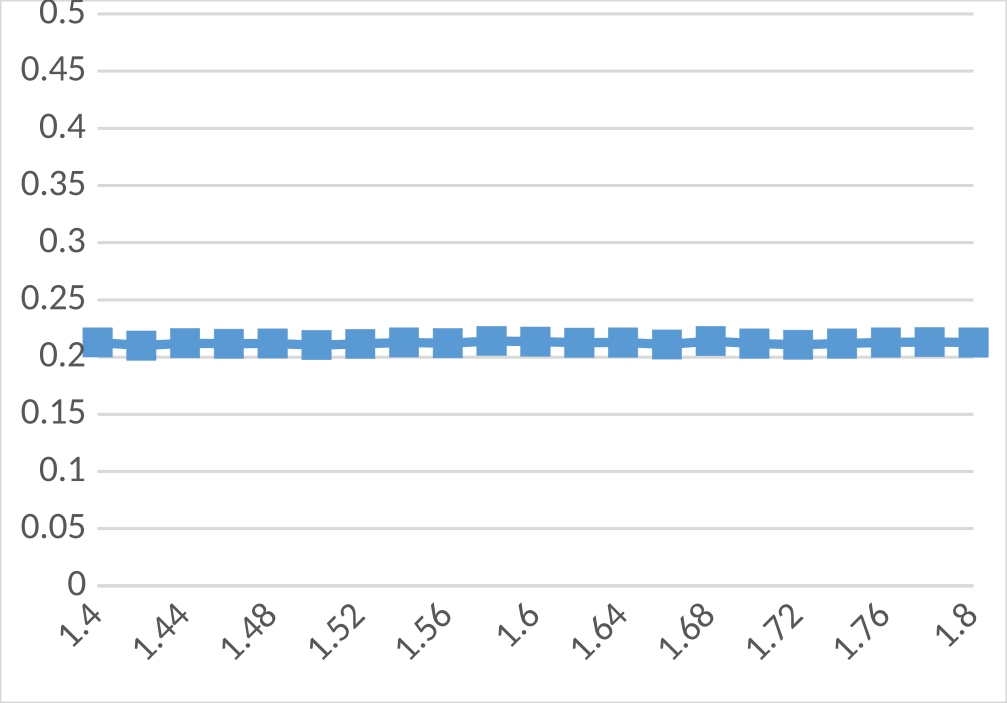
\includegraphics[width=\textwidth]{figs/inv_ql_fifo.png}
    (a)
  \end{minipage}\hspace{0.01\textwidth}
  \begin{minipage}{0.32\textwidth}
    \centering
    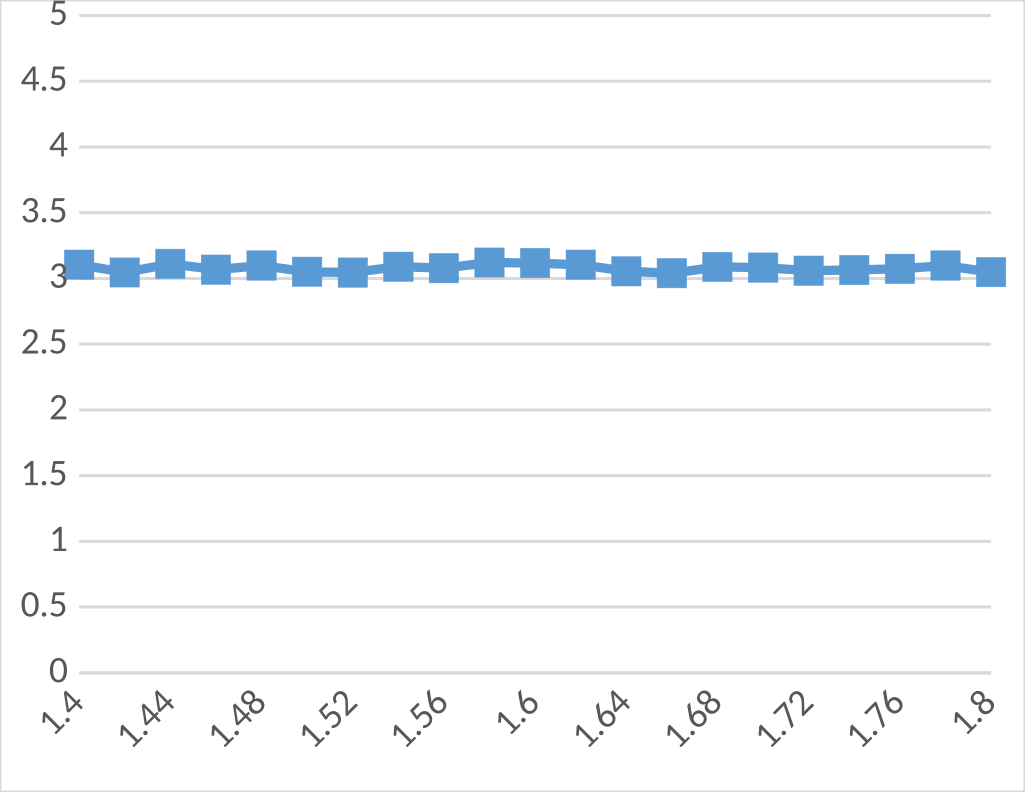
\includegraphics[width=\textwidth]{figs/inv_ql_normal.png}
    (b)
  \end{minipage}\hspace{0.01\textwidth}
  \begin{minipage}{0.32\textwidth}
    \centering
    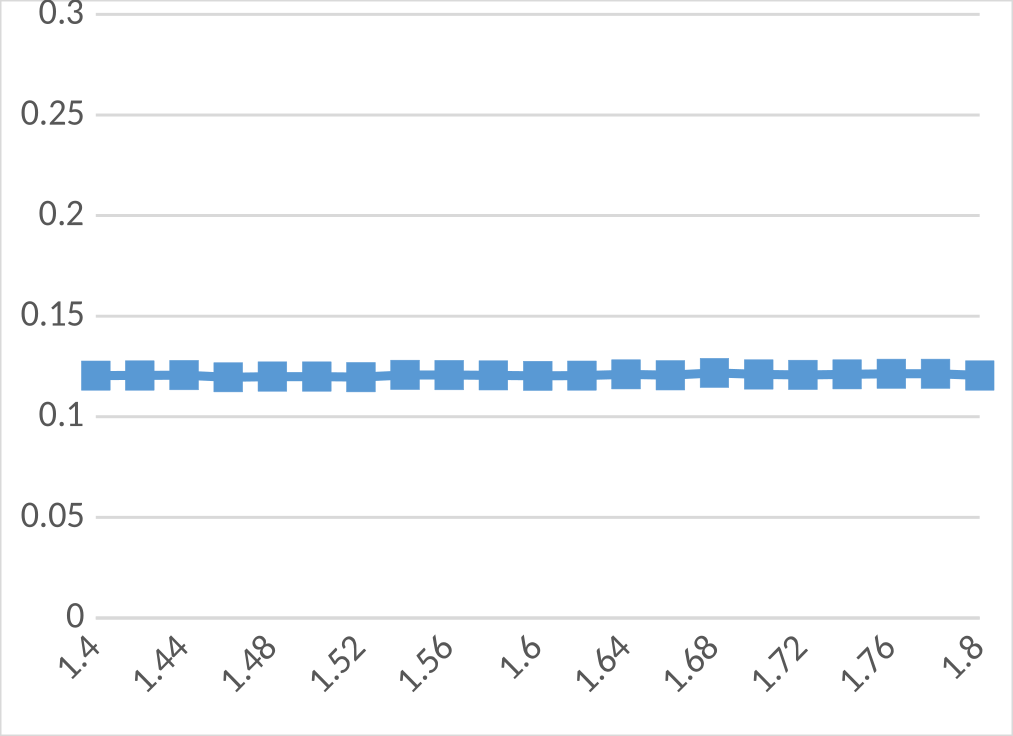
\includegraphics[width=\textwidth]{figs/inv_ql_vip.png}
    (c)
  \end{minipage}
  \caption{Kitchen queue length as a function of the cashier service rate in the FIFO (a) and priority (b: normal queue; c: VIP queue). 
  $r=30,\lambda_N=1,\lambda_V=0.2,\pi_C=0.2,\mu_K=0.3,\mu_C=\{1.4..1.8 \text{ step } 0.02\}$.}
  \label{fig:inv_ql}
\end{figure}

In \cref{sec:2kr} we showed how the kitchen mean queue length was not influenced by the cashier rate and \cref{fig:inv_ql} just confirms the above result. Furthermore, recall that the same result was obtained also in the mathematical model for the FIFO case.

\subsection{``Business day'' analysis}
After having studied the system response at the steady state, we decided to observe it also in a business day. We used the multipliers in \cref{fig:bd:mul} to vary the arrival rate throughout the day so that to have peaks during meal times. In the following section, each scenario has been repeated 100 times and obtained confidence intervals are shown in the plots.

\begin{figure}[H]
  \begin{minipage}{0.48\textwidth}
    \centering
    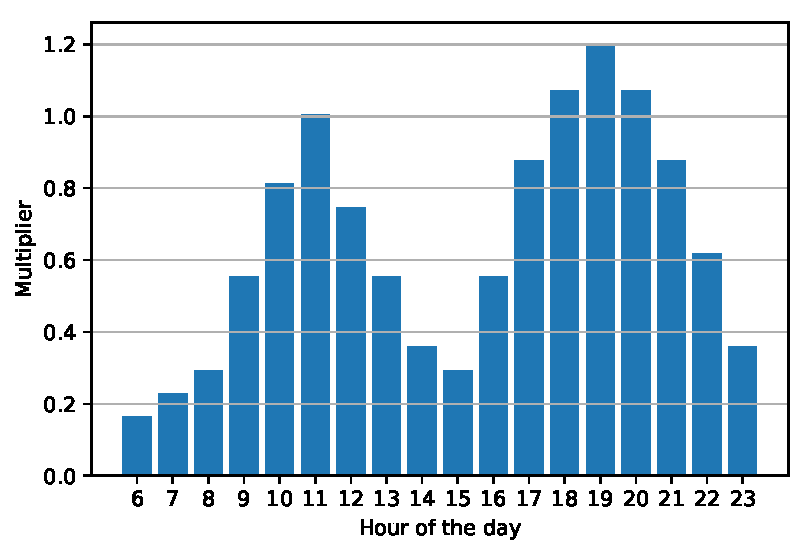
\includegraphics[width=\textwidth]{figs/business_day/input_bd.pdf}
    \caption{Multipliers used to modify the average arrival rate per business hour.}
    \label{fig:bd:mul}
  \end{minipage}\hspace{0.03\textwidth}
  \begin{minipage}{0.48\textwidth}
    \centering
    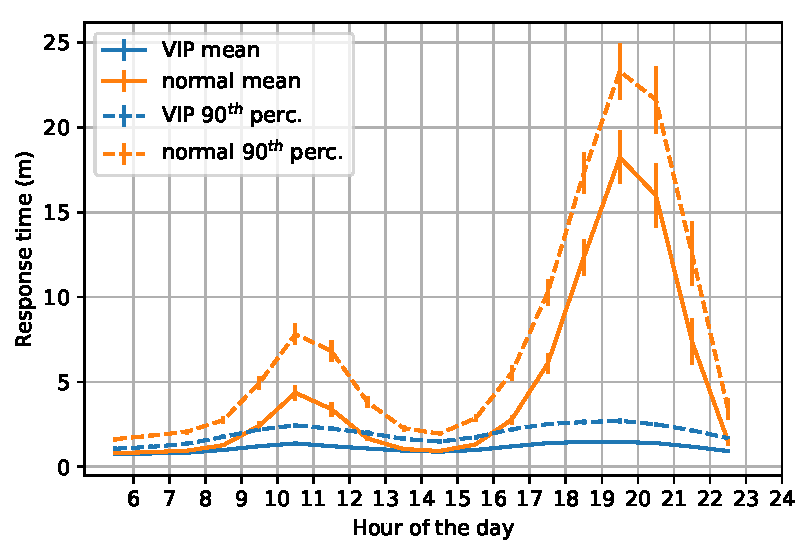
\includegraphics[width=\textwidth]{figs/business_day/vip_vs_normal_simple.pdf}
    \caption{Comparison of the hourly average of the response time for VIP and normal customers with simple orders in a ``normal'' business day ($\mu_C=1.5, \mu_K=0.4, \lambda_{tot,max} = 1.65, \pi_V=0.2, \pi_C=0.2$).}
    \label{fig:bd:vip_vs_norm}
  \end{minipage}
\end{figure}

\cref{fig:bd:vip_vs_norm} shows a comparison between VIP and normal customers. As expected, the VIP customers are serviced very fast and experience almost no waiting time. Furthermore, note that the mean waiting time during dinner is much higher than lunch time since, with the used configuration, during the former the arrival rate exceeds the cashier service rate, conversely to what happens in the latter.

\cref{fig:bd:var_cr,fig:bd:var_ar} show the response of the system when varying, respectively, the cashier rate and the arrival rate. Both plots highlight that a small change ($\sim 10\%$) of either rate leads to an exponential change of the response time. Thus, even a small improvement in cashier speed during peak times could lead to huge improvements in customer satisfaction.

\begin{figure}[H]
  \begin{minipage}{0.48\textwidth}
    \centering
    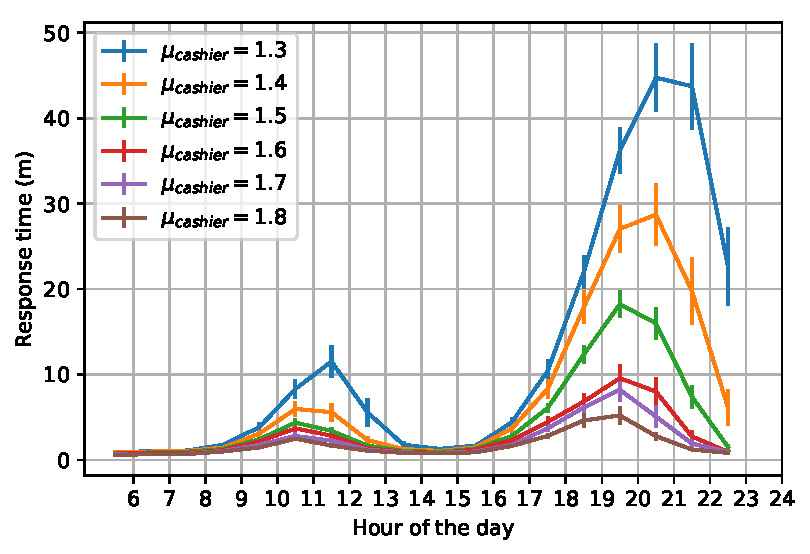
\includegraphics[width=\textwidth]{figs/business_day/varying_cashier_rate.pdf}
    \caption{Hourly average of the response time for normal-simple orders in a business day at different cashier rates ($\mu_K=0.4, \lambda_{tot,max} = 1.65, \pi_V=0.2$).}
    \label{fig:bd:var_cr}
  \end{minipage}\hspace{0.03\textwidth}
  \begin{minipage}{0.48\textwidth}
    \centering
    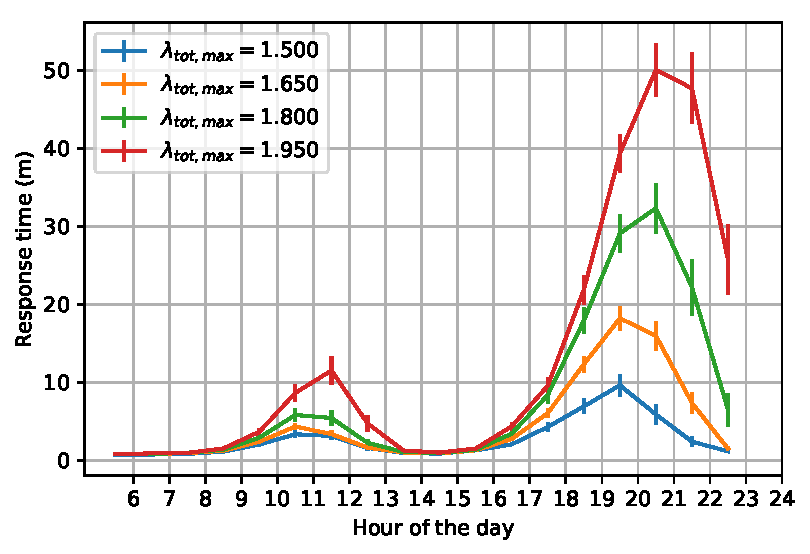
\includegraphics[width=\textwidth]{figs/business_day/varying_arrival_rate.pdf}
    \caption{Hourly average of the response time for normal-simple orders in a business day at different arrival rates ($\mu_C = 1.5, \mu_K=0.4, \pi_V=0.2$).}
    \label{fig:bd:var_ar}
  \end{minipage}
\end{figure}
